\chapter{Sliding Motion Planning Benchmarks}
\label{chap:app-sliding}

The motion planning algorithms presented in Chapter
\ref{chap:wholebody-planning} have been implemented using
KineoWorks\texttrademark \cite{laumond2006kcs}. The planning times
have been measured on an Intel Core~2~Duo 2.13~GHz PC with 2~GB of
RAM. Evaluation of the randomized algorithm has been conducted by
executing 500 trials on each scenario using two flavors of RRT: the
classic RRT and IPP-RRT \cite{FERR04A}. We present the results in
Figures \ref{fig:rrt-it}, \ref{fig:rrt-t} and \ref{fig:rrt-n}.

\begin{figure}[h]
\centering
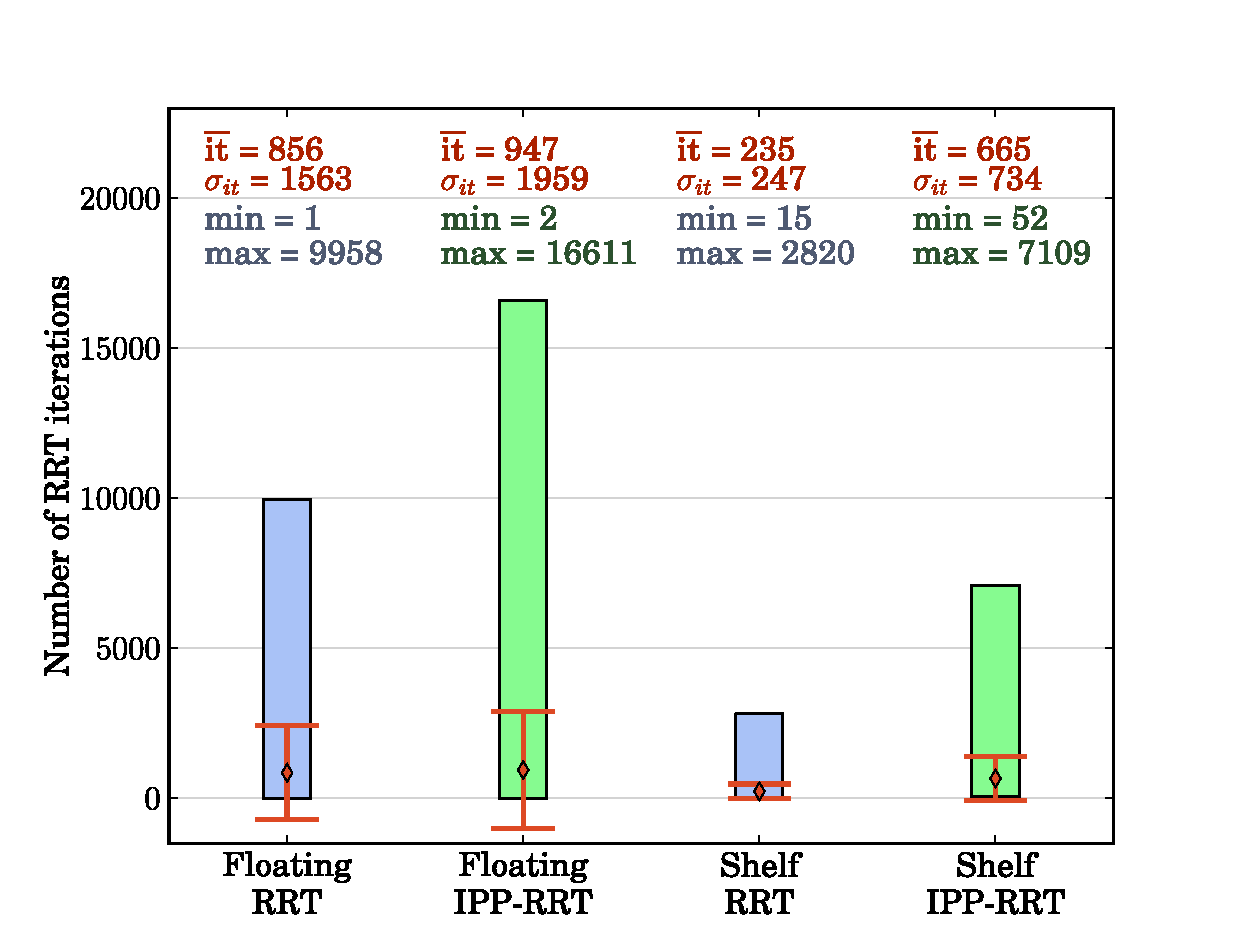
\includegraphics[width=0.7\linewidth]
                {src/appendix/plots/rrt-it.eps}
\caption[Number of RRT iterations for scenarios.]{Number of RRT
  iterations $it$ for the floating objects and the shelf scenarios,
  using two variants of RRT. Mean $\overline{it}$, standard deviation
  $\sigma_{it}$, minimum and maximum values are represented.}
\label{fig:rrt-it}
\end{figure}

\begin{figure}
\centering
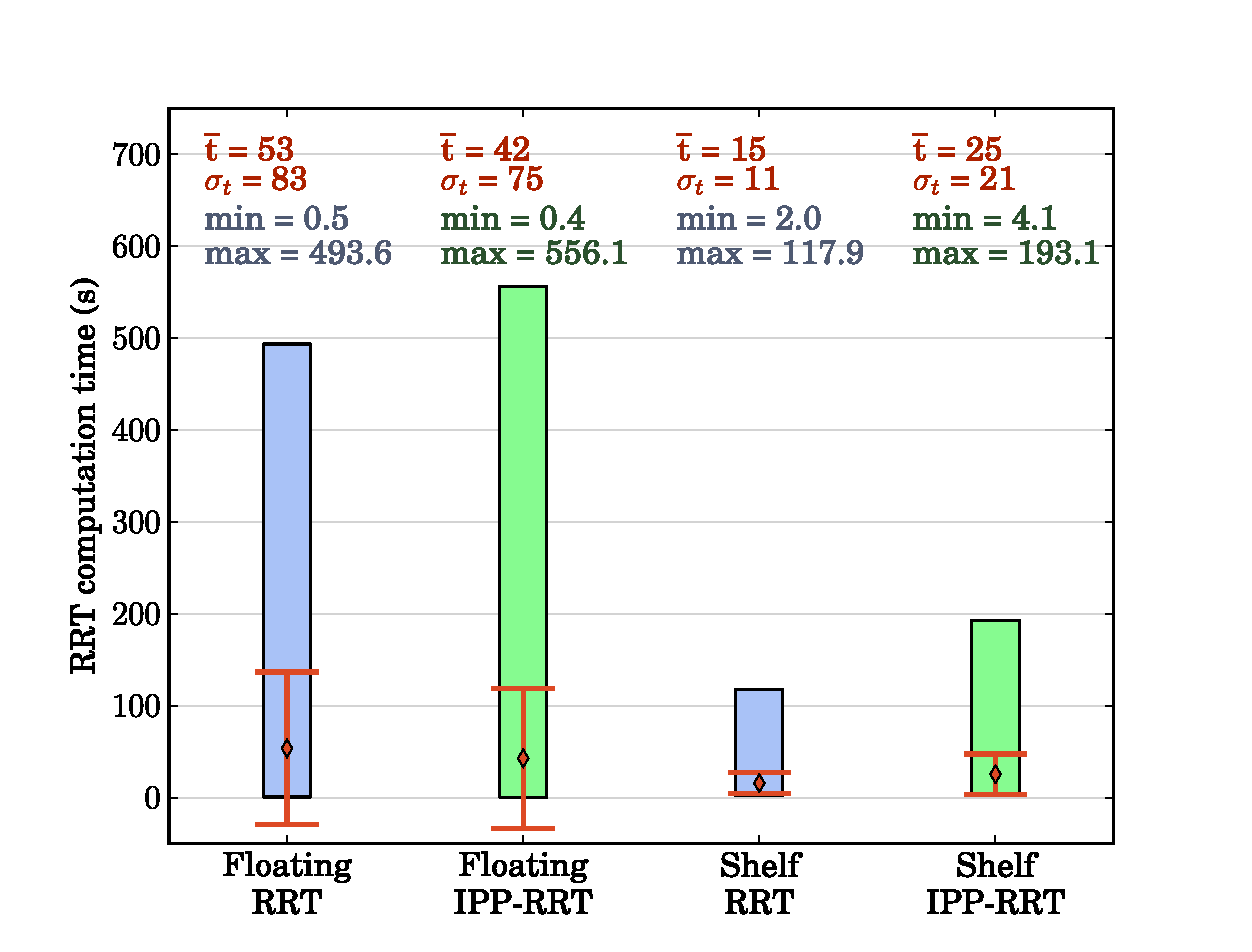
\includegraphics[width=0.7\linewidth]
                {src/appendix/plots/rrt-t.eps}
\caption[RRT computation time for scenarios.]{RRT computation time $t$
  for the floating objects and the shelf scenarios, using two variants
  of RRT. Mean $\overline{t}$, standard deviation $\sigma_{t}$,
  minimum and maximum values are represented.}
\label{fig:rrt-t}
\end{figure}

\begin{figure}
\centering
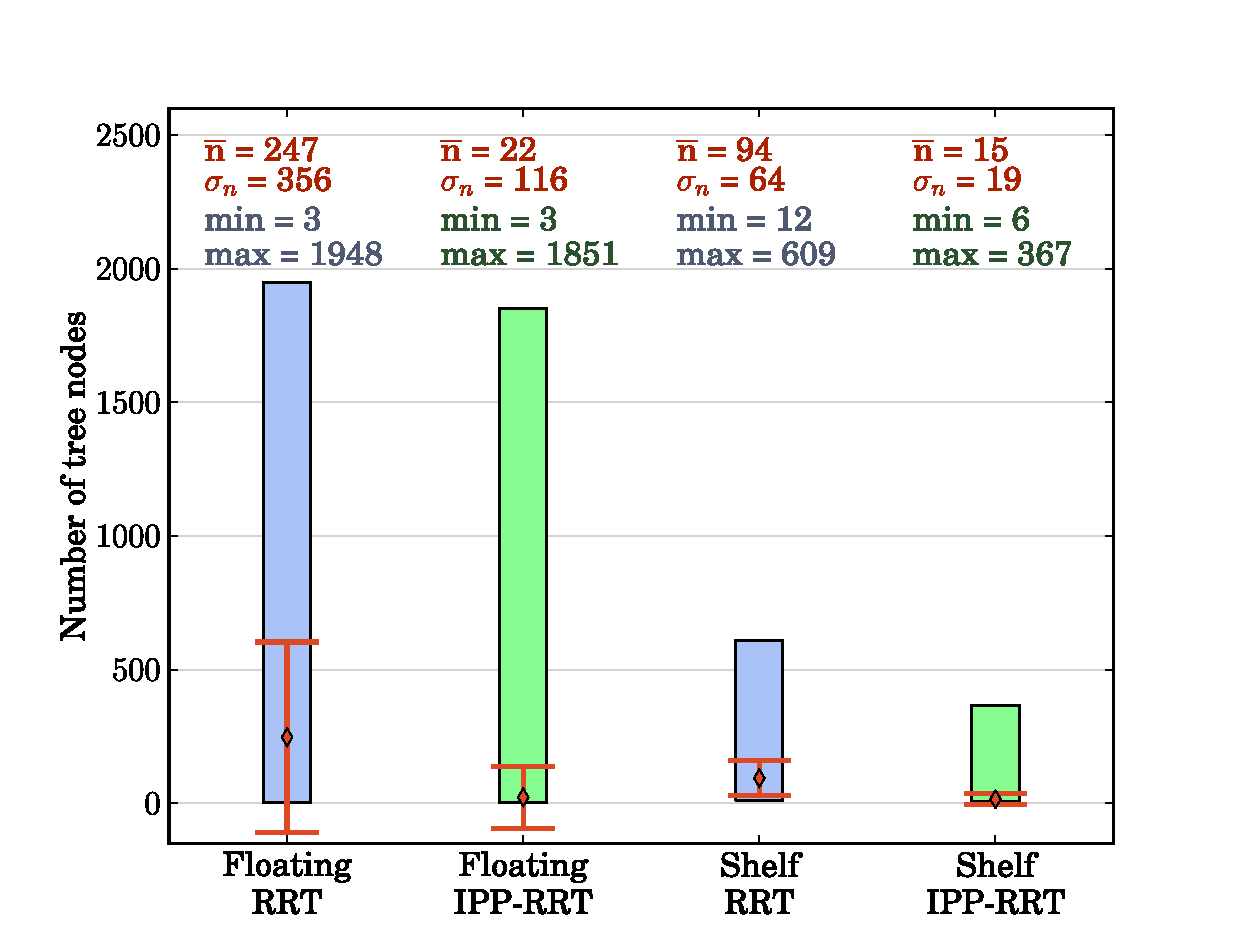
\includegraphics[width=0.7\linewidth]
                {src/appendix/plots/rrt-n.eps}
\caption[Number of tree nodes for scenarios.]{Number of tree nodes $n$
  for the floating objects and the shelf scenarios, using two variants
  of RRT. Mean $\overline{n}$, standard deviation $\sigma_{n}$,
  minimum and maximum values are represented.}
\label{fig:rrt-n}
\end{figure}

\chapter{Numerical Optimization}
\label{chap:app-numerical-optimization}

We give here an overview of the most successful numerical optimization
techniques that can be found in the literature. We focus on
Jacobian-based methods, i.e.\ methods that use information given by the
\emph{variations} of the function we want to minimize to find its
minimizer. As this section is largely based on
\cite{nocedal1999numerical}, we invite the interested reader to refer
to it for more details.

\section{Unconstrained Optimization}

Given a scalar \emph{objective function} $f:\mathbb R^n \rightarrow
\mathbb R$, we would like to solve the following problem:

\begin{equation}
\min_{\mathbf{x}\in\mathbb R^n}f(\mathbf{x})
\end{equation}

This is a problem of \emph{unconstrained optimization}; it consists of
finding one ore more solutions $\argmin{x}$, which we call
\emph{minimizers}. A minimizer is said to be \emph{global} if and only
if:

\begin{equation}
f(\argmin{x}) \le f(\mathbf{x})~\forall \mathbf{x} \in \mathbb R^n,
\end{equation}

\noindent implying that there is no other point $\mathbf{x}\in\mathbb R^n$ such
that the value of $f$ at $\mathbf{x}$ is lower than the value of $f$
at $\argmin{x}$. On the other hand, a \emph{local minimizer} is such
that $\exists$ a neighborhood $\mathcal{N}$ of $\argmin{x}$ and:

\begin{equation}
\label{eq:chap3-local-min}
  f(\argmin{x}) \le f(\mathbf{x})~\forall \mathbf{x} \in \mathcal{N}.
\end{equation}

Obviously, a local minimizer is weaker than a global minimizer, as
Equation \equref{eq:chap3-local-min} implies that there is no other
minimizer only in the vicinity of $\argmin{x}$, and it does not ensure
the nonexistence of another point $\mathbf{x}^\star_g$ such that
$f(\mathbf{x}^\star_g) \le f(\argmin{x})$. Therefore, there is no
guarantee that the local minimizer is also a global one for $f$.

\subsection{Necessary Conditions}

In order to characterize a minimizer of $f$, we introduce the
\emph{first-order necessary conditions} for unconstrained
optimization:

\begin{theorem}
\label{thm:chap3-first-order-cond}
$\argmin{x}$ is a local minimizer, f continuously differentiable
($C^1$) in an open neighborhood of $\argmin{x} \Rightarrow
\nabla f(\argmin{x}) = \mathbf{0}$.
\end{theorem}

All points $\argmin{x}$ which satisfy the first-order conditions are
called stationary points. Note that stationary points can correspond
to minimizers, maximizers, or saddle points of $f$. The
\emph{second-order necessary conditions} are then used to distinguish
local minimizers:

\begin{theorem}
\label{thm:chap3-second-order-cond}
$\argmin{x}$ is a local minimizer, f twice continuously differentiable
($C^2$) in an open neighborhood of $\argmin{x} \Rightarrow \nabla
f(\argmin{x}) = \mathbf{0}$ and $\nabla^2 f(\argmin{x})$ is positive
semi-definite (psd).
\end{theorem}

The key for the conditions is that $f$ be at least $C^2$ so that
$\nabla f$ and $\nabla^2 f$ be defined and continuous. Note that if
$f$ is convex and $C^1$, $\nabla^2 f(x)$ is positive definite (pd)
$\forall~\mathbf{x}$, and it can be shown that any stationary point of
$f$ is also a global minimizer of $f$.

\subsection{Finding the Minimizer}

One way of finding a minimizer of $f$ is to look for a stationary
point starting from an initial point $\arginit{x}$, and produce a
sequence of iterates $\{\mathbf{x}_k\}_{k=0}^{\infty}$ that terminates
when a termination condition is reached; this condition corresponds to
the point $\argmin{x}$ where no more progress can be made, up to a
specified tolerance $\epsilon > 0$.

Given an iterate $\mathbf{x_k}$, the next iterate $\mathbf{x_{k+1}}$
can be chosen based on information about $f$ at $\mathbf{x_k}$ so that
$f(\mathbf{x_{k+1}})<f(\mathbf{x_k})$. There exist two main strategies
to do so:

\begin{enumerate}
\item Line search strategy: a direction $\mathbf{p_k}$ is first
  chosen, then a step length $\alpha_k > 0$ is computed such that it
  approximately solves the 1D minimization problem: $\min_{\alpha>0}
  f(\mathbf{x_k}+\alpha_k\mathbf{p}_k)$. This leads to
  $\mathbf{x}_{k+1}=\mathbf{x}_k+\alpha_k\mathbf{p_k}.$
\item Trust region strategy: a local model $m_k$ of $f$ is
  constructed, and a direction $p_k$ is chosen inside a fixed-size
  trust region such that it approximately solves the minimization
  problem: $\min_{\mathbf{p_k}} m_k(\mathbf{x}_k+\mathbf{p}_k)$.
\end{enumerate}

Note that these two strategies are very similar as they try to find
approximate solutions to simple optimization problems which offer good
performance. They mainly differ in the order in which the step length
and search direction are chosen. In the following section, we describe
some of the most common line search strategies. We illustrate them
using the Rosenbrock function \cite{rosenbrock1960automatic}, or banana
function, defined as:

\begin{equation}
\mathbf{x} = (x,y) \in \mathbb R^2,\quad R(\mathbf{x}) =
(1-x^2)+100(y-x^2)^2.
\end{equation}

$R$ has only one minimizer $\argmin{x} = (1,1)$, and is commonly used
to benchmark optimization algorithms.

\subsection{Steepest Descent Line Search}

Let $f_k$ denote $f(\mathbf{x}_k)$ $\forall~k > 0$. Using a
first-order Taylor approximation of $f$, it can be proved that:
\begin{equation}
\mathbf{p_k} = -\nabla f_k
\end{equation}
\noindent is the steepest descent direction, i.e.\ it is the direction along
which $f$ decreases the most locally around $\mathbf{x}_k$.

This strategy has a \emph{linear convergence rate}:
\begin{equation}
\frac{\norm{\mathbf{x}_{k+1}-\argmin{x}}}{\norm{\mathbf{x}_k-\argmin{x}}}
\le r \text{ for all } k \text{ sufficiently large}, \quad
r=\frac{\kappa-1}{\kappa+1},
\end{equation}

\noindent where $\kappa$ is the condition number of the Hessian
$\nabla^2 f$, i.e.\ the ratio of the maximum singular value over the
minimum singular value of $\nabla^2 f$.  It can therefore lead to
extremely slow convergence when $\nabla^2 f$ is ill-conditioned and $r
\approx 1$.

Figure \ref{fig:chap3-unconstrained-steepest-descent} shows an example
of minimizing the Rosenbrock function. We show the first 20 iterates
when using a steepest descent line search and setting $\alpha_k$ to a
constant value of 1. The search direction $\mathbf{p_k}$ is always
orthogonal to the function contour line, as it is the direction that
allows to decrease $R$ quickly. Unfortunately, as the iterates reach
the basin, keeping a constant step size leads to a strong oscillation
and convergence is not achieved. This motivates the need for a good
step size computation method that will ensure a decrease of the
function at each iteration.

\begin{figure}
  \centering
      {\def\svgwidth{0.8\linewidth}
        {\footnotesize
          \subimport*{src/chap3-optimal-motion-planning/figure/}
                     {unconstrained-steepest-descent.pdf_tex}
        }
      }
      \caption[Steepest descent line search.]{Contour lines show the
        Rosenbrock function $R$. Starting from
        $\arginit{x}=(-0.6,-0.6)$, a steepest descent line search is
        used with a constant step size $\alpha_k=1$. The minimizer
        basin is reached very quickly, but large values of the step
        size then prevent minimizing the function. Note that the
        steepest descent direction is orthogonal to the contour lines
        of $R$.}
      \label{fig:chap3-unconstrained-steepest-descent}
\end{figure}

The Wolfe conditions offer the theoretical means and an easily
verifiable way to compute suitable step lengths. They are defined as:

\begin{equation}
\label{eq:chap3-wolfe-1}
f(\mathbf{x}_k + \alpha_k\mathbf{p}_k) \le
f(\mathbf{x_k}+c_1\alpha_k\nabla f_k^{\top}\mathbf{p_k}),
\end{equation}
\begin{equation}
\label{eq:chap3-wolfe-2}
\nabla f(\mathbf{x_k} + \alpha_k
\mathbf{p}_k)^{\top}\mathbf{p_k} \ge c_2 \nabla f_k^{\top}\mathbf{p_k},
\end{equation}

\noindent where $0 < c_1 < c_2 < 1$. Equation
\equref{eq:chap3-wolfe-1} is called the \emph{sufficient decrease} or
\emph {Armijo condition}; it rejects too small decreases in
$f$. Equation \equref{eq:chap3-wolfe-2} is called the \emph{curvature
  condition}, and it rejects too negative slopes which might slow down
convergence. In practice, $c_1$ is very small and set to $10^{-4}$,
while $c_2$ is set to a value ranging from $0.1$ to $0.9$.

The Wolfe conditions can be used to write a simple step length
computation algorithm, as described in
Algorithm~\ref{alg:chap3-line-search-wolfe}. The idea is to start with
a large value of $\alpha_k$ and decrease it until the Wolfe conditions
are satisfied.

\begin{algorithm}
\caption{\texttt{StepLengthWolfe}($f$, $\mathbf{x}_k$, $\mathbf{p}_k$,
  $\alpha_k$, $\rho$, $it\_max$)}
\label{alg:chap3-line-search-wolfe}
\begin{algorithmic}
\STATE $it$ $\leftarrow$ $0$
\WHILE{Wolfe conditions are not verified \& $it < it\_max$}
\STATE {\color{red} // $\rho < 1$}
\STATE $\alpha_k$ $\leftarrow$ $\rho \alpha_k$ 
\STATE $it$ $\leftarrow$ $it + 1$
\ENDWHILE
\RETURN $\alpha_k$
\end{algorithmic}
\end{algorithm}

Figure \ref{fig:chap3-unconstrained-steepest-descent-wolfe} shows the
solution to the same problem as in Figure
\ref{fig:chap3-unconstrained-steepest-descent} with the Wolfe
conditions enforced at each iteration. The minimizer
$\argmin{x}=(1~1)$ is reached after around 5000 iterations. Such a
high number is mainly due to an ill-conditioned Hessian and the
induced zigzagging behavior which prevents quickly reaching the
minimizer, as shown in Figure
\ref{fig:chap3-unconstrained-steepest-descent-wolfe-b}.

\begin{figure}
  \setlength{\belowcaptionskip}{\baselineskip}
  \centering
  \begin{subfigure}{0.8\columnwidth}
    \centering
        {\def\svgwidth{\linewidth}
          {\footnotesize
            \subimport*{src/chap3-optimal-motion-planning/figure/}
                       {unconstrained-steepest-descent-wolfe.pdf_tex}
          }
        }
        \caption{Solution to the Rosenbrock function minimization
          problem.}
        \label{fig:chap3-unconstrained-steepest-descent-wolfe-a}
  \end{subfigure}
  \begin{subfigure}{0.8\columnwidth}
    \centering
        {\def\svgwidth{\linewidth}
          {\footnotesize
            \subimport*{src/chap3-optimal-motion-planning/figure/}
                       {unconstrained-steepest-descent-wolfe-zoom.pdf_tex}
          }
        }
        \caption{Enlarged view: the zigzagging behavior slows down
          convergence.}
        \label{fig:chap3-unconstrained-steepest-descent-wolfe-b}
  \end{subfigure}
  \caption[Steepest-descent line search strategy with Wolfe
    conditions.]{Steepest-descent line search strategy. The Wolfe
    conditions are enforced at each iteration to ensure sufficient
    decrease of the objective function.}
  \label{fig:chap3-unconstrained-steepest-descent-wolfe}
\end{figure}

\subsection{Newton Line Search}

Assuming that $f$ is $C^2$ and using a second-order Taylor
approximation at $\mathbf{x}_k$, we can derive the \emph{Newton
  direction}:
\begin{equation}
\mathbf{p_k} = -\nabla^2 f_k^{-1} \nabla f_k;
\end{equation}
$\mathbf{x}_{k+1}=\mathbf{x_k}+\mathbf{p_k}$ is then the minimizer of
the local quadratic approximation of $f$. The Newton direction has a
natural step length $\alpha_k=1$. Nevertheless the Wolfe conditions
still need to be verified to make sure that there is a decrease in the
exact function $f$. Figure \ref{fig:chap3-unconstrained-newton-wolfe}
shows the sequence of iterates when applying a Newton line search to
find the minimizer of the Rosenbrock function. It is clear in Figure
\ref{fig:chap3-unconstrained-newton-wolfe-quad} how the next iterate
is the minimizer of the local quadratic approximation of the objective
function.

\begin{figure}
  \setlength{\belowcaptionskip}{\baselineskip}
  \centering
  \begin{subfigure}{0.8\columnwidth}
    \centering
        {\def\svgwidth{\linewidth}
          {\footnotesize
            \subimport*{src/chap3-optimal-motion-planning/figure/}
                       {unconstrained-newton-wolfe.pdf_tex}
          }
        }
        \caption{Solution to the Rosenbrock
          function minimization problem: a few iterations are needed
          to find the minimizer $\argmin{x}$.}
        \label{fig:chap3-unconstrained-newton-wolfe-a}
  \end{subfigure}
  \begin{subfigure}{0.8\columnwidth}
    \centering
        {\def\svgwidth{\linewidth}
          {\footnotesize
            \subimport*{src/chap3-optimal-motion-planning/figure/}
                       {unconstrained-newton-wolfe-quad.pdf_tex}
          }
        }
        \caption{The contour lines show the local quadratic
          approximation of $R$ around $\arginit{x}$. The next iterate
          $\argmin{x}_1$ is then the minimizer of the quadratic
          approximation.}
        \label{fig:chap3-unconstrained-newton-wolfe-quad}
  \end{subfigure}
  \caption[Newton line search.]{Newton line search. The Wolfe
    conditions are enforced at each iteration to ensure sufficient
    decrease of the objective function.}
  \label{fig:chap3-unconstrained-newton-wolfe}
\end{figure}

The Newton line search is very efficient and exhibits a
\emph{quadratic convergence rate}:

\begin{equation}
\frac{\norm{\mathbf{x}_{k+1}-\argmin{x}}}{\norm{\mathbf{x}_k-\argmin{x}}^2}
\le M \text{ for all } k \text{ sufficiently large}, \quad M>0,
\end{equation}

\noindent which is faster than a linear convergence rate. However, beside
knowing how to compute the Jacobian of $f$, we also need to derive the
Hessian of $f$ and this is not always a trivial task.

\subsection{Quasi-Newton Line Search}
\label{subsubsec:chap3-quasi-newton-line-search}

Instead of using the Hessian, a quasi-Newton line search relies on an
approximation of $\nabla^2 f$ when it is not possible to compute
it. The search direction is then given by:
\begin{equation}
p_k=-\mathbf{B}_k^{-1}\nabla f_k,
\end{equation}
\noindent where $\mathbf{B}_k\approx\nabla^2 f$ is a symmetric nonsingular
matrix.

\begin{algorithm}
\caption{\texttt{BFGS}($\arginit{x}$, $\epsilon$)}
\label{alg:chap3-bfgs}
\begin{algorithmic}
\STATE $\mathbf{H}_0$ $\leftarrow$ $\mathbf{I}$, $k$ $\leftarrow$ $0$
\WHILE{$\norm{\nabla f_k} > \epsilon$}
\STATE {\color{red} // Search direction}
\STATE $\mathbf{p}_k$ $\leftarrow$ $-\mathbf{H}_k\nabla f_k$
\STATE {\color{red} // Line search with Wolfe conditions}
\STATE $\mathbf{x}_{k+1}$ $\leftarrow$ $\mathbf{x}_k + \alpha_k\mathbf{p}_k$
\STATE $\mathbf{s}_k$ $\leftarrow$ $\mathbf{x}_{k+1} - \mathbf{x}_k$
\STATE $\mathbf{y}_k$ $\leftarrow$ $\nabla f_{k+1} - \nabla f_k$
\STATE $\rho_k$ $\leftarrow$ $\frac{1}{\mathbf{y}_k^{\top}\mathbf{s}_k}$
\STATE {\color{red} // BFGS update of the Hessian inverse}
\STATE $\mathbf{H}_{k+1}$ $\leftarrow$ $(\mathbf{I}-\rho_k\mathbf{s}_k\mathbf{y}_k^{\top})\mathbf{H}_k(\mathbf{I}-\rho_k\mathbf{y}_k\mathbf{s}_k^{\top})+\rho_k\mathbf{s}_k\mathbf{s}_k^{\top}$
\STATE $k$ $\leftarrow$ $k + 1$
\ENDWHILE
\end{algorithmic}
\end{algorithm}

Several algorithms for deriving approximates $\mathbf{B_k}$ exist, the
best one being the Broyden-Fletcher-Goldfarb-Shanno (BFGS) method, as
described in Algorithm \ref{alg:chap3-bfgs}. It relies on updating the
$\mathbf{H}_k = \mathbf{B}_k^{-1}$ while the iterative optimization is
taking place. As an initial value $\mathbf{H}_0=\mathbf{I}$ is given,
the line search behaves like a steepest-descent line search for the
first iterations, converging towards a Newton line search as the
optimization advances and as the approximation is closer to the real
Hessian. The BFGS line search has then a \emph{superlinear
  convergence rate}:

\begin{equation}
\underset{k\rightarrow\infty}{\text{lim}}
\frac{\norm{\mathbf{x}_{k+1}-\argmin{x}}}{\norm{\mathbf{x}_k-\argmin{x}}}
= 0,
\end{equation}

\begin{figure}
  \centering
      {\def\svgwidth{0.8\linewidth}
        {\footnotesize
          \subimport*{src/chap3-optimal-motion-planning/figure/}
                     {unconstrained-quasi-newton-wolfe.pdf_tex}
        }
      }
      \caption[Quasi-Newton line search.]{Rosenbrock function
        minimization with a quasi-Newton line search using a
        BFGS-Hessian approximation. It is interesting to note that the
        line search behaves like a steepest-descent line search for
        the first iterations, converging towards a Newton line
        search.}
      \label{fig:chap3-unconstrained-quasi-newton-wolfe}
\end{figure}

\subsection{Constrained Optimization}

The previous section described methods that allow us to solve the
problem of unconstrained optimization, which consists in finding the
minimizer $\argmin{x}\in\mathbb R^n$ of a scalar function $f$. In many
cases, however, the minimizer is required to additionally obey to a
number of \emph{constraints} in order to be feasible. The general
\emph{constrained optimization} problem can then be written as:

\begin{equation}
\label{eq:chap3-nlp}
\min_{\mathbf{x} \in \mathbb R^n}
f(\mathbf{x}),\text{ such that }
\left\{\begin{array}{cc}
c_i(\mathbf{x}) = 0, & i \in \mathcal{E} \\%
c_i(\mathbf{x}) \ge 0, & i \in \mathcal{I} %
\end{array}\right.
\end{equation}

$\Omega=\{\mathbf{x}\in\mathbb R^n: c_i(\mathbf{x}) = 0, i \in
\mathcal{E}; c_i(\mathbf{x}) \ge 0, i \in \mathcal{I}\}$ is called the
\emph{feasible set}, and a point $\mathbf{x}$ is said to be feasible
iff $\mathbf{x}\in\Omega$. At a feasible point, an inequality
constraint $c_i~(i\in \mathcal{I})$ is:

\begin{itemize}[noitemsep,nolistsep]
\item active iff $c_i(\mathbf{x})=0$, i.e.\ $\mathbf{x}$ is on the boundary of $c_i$,
\item inactive iff $c_i(\mathbf{x})>0,$ i.e.\ $\mathbf{x}$ is an
  interior point of $c_i$.
\end{itemize}
\vspace{\baselineskip}
We can then define the active set at $\mathbf{x}$:

\begin{equation}
\mathcal{A}(\mathbf{x})=\mathcal{E}\cup\{i\in\mathcal{I}:c_i(\mathbf{x}=0)\},
\end{equation}

\noindent as the set of all active constraints at a point $\mathbf{x}$. Let us
also define the active constraint gradients at $\mathbf{x}$:

\begin{equation}
\mathbf{A}(\mathbf{x})=\left[\nabla
  c_i(\mathbf{x})\right]_{i\in\mathcal{A}(\mathbf{x})}^\top
\end{equation}

The optimality conditions we introduced in Theorems
\ref{thm:chap3-first-order-cond} and \ref{thm:chap3-second-order-cond}
do not hold anymore as we need to take constraints into account. Let
us define the \emph{Lagrangian}:

\begin{equation}
\mathcal{L}(\mathbf{x},\boldsymbol{\lambda}) =
f(\mathbf{x})-\sum_{i\in\mathcal{E}\cup\mathcal{I}}
\lambda_ic_i(\mathbf{x}),
\end{equation}

\noindent where $\lambda_i,~i\in \mathcal{E}\cup\mathcal{I}$ are called the
\emph{Lagrange multipliers}.

It can be shown that candidate minimizers are the stationary points of
$\mathcal{L}$, which is equivalent to $\nabla f$ lying in the subspace
spanned by the active constraint gradients $\nabla
c_i,~i\in\mathcal{A(\mathbf{x})}$. The components of $\nabla f$
expressed in this subspace basis correspond then to the active
constraint Lagrange multipliers
$\lambda_i,~i\in\mathcal{A}(\mathbf{x})$. This leads to the
\emph{Karush-Kuhn-Tucker (KKT) first-order necessary conditions}:

\begin{theorem}
\label{eq:chap3-kkt}
$\argmin{x}$ is a local minimizer, f is $C^1$ in an open neighborhood
of $\argmin{x}$, $\mathbf{A}(\mathbf{x})$ is full-rank $\Rightarrow$
$\exists! \boldsymbol{\lambda}^{\star} \in \mathbb R^m$ such that:
\[
\begin{array}{crcl}
a) & \nabla_{\mathbf{x}}\mathcal{L}(\argmin{x}, \boldsymbol{\lambda}^\star) & = & \mathbf{0} \\%
b) & c_i(\argmin{x}) & = & 0 \qquad \forall i \in \mathcal{E} \\%
c) & c_i(\argmin{x}) & \ge & 0 \qquad \forall i \in \mathcal{I}\\%
d) & \lambda_i^{\star} & \ge & 0 \qquad \forall i \in \mathcal{I}\\%
e) & \lambda_i^{\star} c_i(\argmin{x}) & = & 0 \qquad \forall i \in \mathcal{E}\cup\mathcal{I}%
\end{array}
\]
\end{theorem}

Note that $f(\argmin{x}) = \mathcal{L}(\argmin{x},
\boldsymbol{\lambda}^\star)$ because of the complementarity condition
$e)$ in Equation \equref{eq:chap3-kkt}.

\section{Quadratic Programming}

In order to find points which satisfy the KKT conditions, we first
consider the simpler problem of \emph{Quadratic programming (QP)},
where the objective function is quadratic, and all constraints are
linear:

\begin{equation}
\label{eq:chap3-qp}
\min_{\mathbf{x} \in \mathbb R^n}
q(\mathbf{x})=\frac{1}{2}\mathbf{x}^{\top}\mathbf{G}\mathbf{x}
+\mathbf{c}^{\top}\mathbf{x},\text{ such that }
\left\{\begin{array}{cc}
\mathbf{a}_i^{\top}\mathbf{x} = b_i, & i \in \mathcal{E} \\%
\mathbf{a}_i^{\top}\mathbf{x} \ge b_i, & i \in \mathcal{I} %
\end{array}\right. ~\mathbf{G}\text{ symmetric.}
\end{equation}

\subsection{Equality-constrained QP}

In the particular case of an equality-constrained QP, we have:

\begin{equation}
\label{eq:chap3-qp-eq}
\min_{\mathbf{x} \in \mathbb R^n}
q(\mathbf{x})=\frac{1}{2}\mathbf{x}^{\top}\mathbf{G}\mathbf{x}
+\mathbf{c}^{\top}\mathbf{x},\text{ such that }
\mathbf{A}\mathbf{x} = b
\qquad \mathbf{A} \text{ full rank.}
\end{equation}

The KKT conditions given in Theorem \equref{eq:chap3-kkt} imply that the
solution $\argmin{x}$ verifies:

\begin{equation}
  \label{eq:chap3-qp-kkt}
  \left(\begin{matrix}
    \mathbf{G} & -\mathbf{A}^{\top} \\
    \mathbf{A} & \mathbf{0}
  \end{matrix}\right)
  \left(\begin{matrix}
    \argmin{x} \\
    \boldsymbol{\lambda}^{\star}
  \end{matrix}\right)
  = \left(\begin{matrix}
    -\mathbf{c} \\
    \mathbf{b}
  \end{matrix}\right)  
  \overset{\argmin{x}=\mathbf{x}+\mathbf{p}}\Longleftrightarrow
  \left(\begin{matrix}
    \mathbf{G} & \mathbf{A}^{\top} \\
    \mathbf{A} & \mathbf{0} \\
  \end{matrix}\right)
  \left(\begin{matrix}
    -\mathbf{p} \\
    \boldsymbol{\lambda}^{\star}
  \end{matrix}\right)
  = \left(\begin{matrix}
    \mathbf{g} \\
    \mathbf{h}
  \end{matrix}\right)
  \quad
  \left\{\begin{matrix}
      \mathbf{h} = \mathbf{A}\mathbf{x} - \mathbf{b} \\
      \mathbf{g} = \mathbf{c} + \mathbf{G}\mathbf{x} \\
      \mathbf{p} = \argmin{x} - \mathbf{x}
    \end{matrix}\right.
\end{equation}

The final linear system in Equation \equref{eq:chap3-qp-kkt} is called
the \emph{KKT system}. It can be solved using standard linear algebra
techniques, and its solution gives the update $\mathbf{p}$ which leads
directly to the minimizer $\argmin{x}$ of $q$.

\begin{figure}
  \centering {\def\svgwidth{0.8\linewidth} {\footnotesize
      \subimport*{src/chap3-optimal-motion-planning/figure/}
                 {qp-equality.pdf_tex} } }
      \caption[Solution of a constrained QP problem.]{Solution of a
        constrained QP problem. One linear equality constraint is
        used, and solutions for different values of the constraint are
        shown. Note that the farther the constraint is from the
        unconstrained minimum, the larger is the associated Lagrange
        multiplier.}
      \label{fig:chap3-qp-equality}
\end{figure}

We use this method to solve an equality-constrained QP, shown in
Figure \ref{fig:chap3-qp-equality}: for the same quadratic objective
function, we find the minimizer for three different linear equality
constraints. We can see that the associated Lagrange multiplier is
higher as the constrained minimizer is further from the unconstrained
minimum. Intuitively, Lagrange multiplier give an idea of the
``force'' which the constraints are exerting on the constrained
minimizer to keep it away from the unconstrained minimum.

\subsection{Inequality-Constrained QP}

Now that we can solve an equality-constrained QP, we can move on to
solve the general QP presented in Equation
\equref{eq:chap3-qp}. Several types of method such as active-set,
gradient-projection and interior-point can be used to this end. We
describe here the active-set method for solving inequality-constrained
QP.

The active-set method, described in detail in Algorithm
\ref{alg:chap3-active-set}, consists in iteratively estimating the
optimal active set, solving the underlying equality-constrained QP
with the active constraints, and repeat until the optimal active set
is correctly found. We implement an active-set method to solve a QP as
shown in Figure \ref{fig:chap3-qp-inequality}. One linear equality
constraint and two linear inequality constraints are added. Starting
from a point $\arginit{x}$, the optimal solution and active set are
found iteratively.

\begin{algorithm}
\caption{\texttt{ActiveSetSolve}($\arginit{x}$)}
\label{alg:chap3-active-set}
\begin{algorithmic}
\STATE {\color{red} // Initialize active set}
\STATE $\mathcal{W}_0$ $\leftarrow$ subset of the active constraints at $\arginit{x}$
\FOR{$k=0,1,2,...$}
\STATE {\color{red} // Find minimizer of equality-constrained QP using active constraints}
\STATE $(\mathbf{p_k}~\boldsymbol{\lambda}_{k+1})$ $\leftarrow$ \texttt{SolveKKTSystem}($\mathbf{W_k}$)
\IF{$\mathbf{p}_k=\mathbf{0}$}
\IF{$\lambda_{k+1,i} \ge 0~\forall i \in \mathcal{W}_k\cap\mathcal{I}$}
\STATE {\color{red} // All inequality constraints in the active set are active}
\RETURN ($\mathbf{x}_k,\boldsymbol{\lambda}_{k+1)}$
\ELSE
\STATE {\color{red} // At least one inequality constraint in the active set is inactive}
\STATE {\color{red} // Remove the one that is ``least active''}
\STATE $\mathcal{W}_{k+1}$ $\leftarrow$ $\mathcal{W}_k \backslash \{\text{arg}\min_{j\in\mathcal{W}_k\cap\mathcal{I}}\lambda_{k+1,j}\}$
\ENDIF
\ELSE
\STATE {\color{red} // Compute $\alpha_k$ such that the constraints which are \emph{not} in the active set are not violated}
\STATE $\alpha_k$ $\leftarrow$ $\min_{\substack{i\notin\mathcal{W}_k\\\mathbf{a}_i^{\top}\mathbf{p}_k<0}} \frac{b_i-\mathbf{a}_i^{\top}\mathbf{x}_k}{\mathbf{a}_i^{\top}\mathbf{p}_k}$
\STATE $\mathbf{x}_{k+1}$ $\leftarrow$ $\alpha_k\mathbf{p}_k$
\IF{$\alpha_k<1$}
\STATE {\color{red} // At least one constraint which is not the active set is active, add one}
\STATE $\mathcal{W}_{k+1}$ $\leftarrow$ $\mathcal{W}_k\cup\{$one blocking constraint$\}$
\ELSE
\STATE {\color{red} // Keep the same active set}
\STATE $\mathcal{W}_{k+1}$ $\leftarrow$ $\mathcal{W}_k$
\ENDIF
\ENDIF
\ENDFOR
\end{algorithmic}
\end{algorithm}

\begin{figure}
  \centering
      {\def\svgwidth{0.8\linewidth}
        {\footnotesize
          \subimport*{src/chap3-optimal-motion-planning/figure/}
                     {qp-inequality.pdf_tex}
        }
      }
      \caption[Solution to the general QP problem using an active-set
        method.]{Solution to the general QP problem using an
        active-set method. The blue line represents the linear
        equality constraint, while the green and red half-planes
        represent the linear inequalities (the infeasible set is
        filled). Starting from $\arginit{x}$, the optimal solution
        $\argmin{x}$ and active set are found iteratively.}
      \label{fig:chap3-qp-inequality}
\end{figure}

\section{Nonlinear Programming}

We are now ready to tackle \emph{Nonlinear programming (NLP)}, i.e.\ to
solve the general problem from Equation \equref{eq:chap3-nlp}. Two of the
most successful methods used nowadays to solve large-scale problems
are \emph{Sequential Quadratic Programming (SQP)} and
\emph{Interior-Point Methods (IPM)}.

\subsection{Sequential Quadratic Programming}
\label{subsubsec:chap3-sqp}

The idea behind SQP is quite simple: for each SQP iteration, we build
a local quadratic approximation of the objective function and
linearized approximation of the constraints in order to obtain a
\emph{QP subproblem}:

\begin{equation}
\label{eq:chap3-sqp}
\begin{array}{c}
\min_{\mathbf{p}}\frac{1}{2}\mathbf{p}_k^{\top}\nabla_{\mathbf{x}\mathbf{x}}^2\mathcal{L}(\mathbf{x}_k,\boldsymbol{\lambda}_k)\mathbf{p}_k+\nabla f(\mathbf{x}_k)^{\top}\mathbf{p}_k+f(\mathbf{x}_k)
\\
\text{ s.t.}
\left\{\begin{array}{cc}
\nabla c_i(\mathbf{x}_k)^{\top}\mathbf{p}_k+c_i(\mathbf{x}_k) = 0, & i \in \mathcal{E} \\
\nabla c_i(\mathbf{x}_k)^{\top}\mathbf{p}_k+c_i(\mathbf{x}_k) \ge 0, & i \in \mathcal{I}
\end{array}\right.
\end{array}
\end{equation}

We then solve the QP subproblem, with active-set methods for instance,
and repeat iteratively until the convergence test is satisfied, as
described in Algorithm~\ref{alg:chap3-sqp}.

\begin{algorithm}
\caption{\texttt{SQPSolve}($\arginit{x}$,$\boldsymbol{\lambda}_0$, $\epsilon$)}
\label{alg:chap3-sqp}
\begin{algorithmic}
\FOR{$k=0,1,2,...$}
\STATE Evaluate $f_k$, $\nabla f_k$, $c_i(\mathbf{x}_k)$, $\nabla c_i(\mathbf{x}_k)$, $\nabla_{\mathbf{x}\mathbf{x}}^2\mathcal{L}(\mathbf{x}_k,\boldsymbol{\lambda}_k)$
\STATE $(\mathbf{p}_k, \boldsymbol{\lambda}_{k+1})$ $\leftarrow$ \texttt{ActiveSetSolve}($\mathbf{x}_k$)
\STATE $\mathbf{x}_{k+1}$ $\leftarrow$ $\mathbf{x}_k + \alpha_k\mathbf{p}_k$
\IF{convergence test satisfied for tolerance $\epsilon$}
\RETURN $(\mathbf{x}_{k+1},\boldsymbol{\lambda}_{k+1})$
\ENDIF
\ENDFOR
\end{algorithmic}
\end{algorithm}

This requires us to derive the Hessian of both objective function and
constraints, see Equation \equref{eq:chap3-sqp}. One solution to avoid
computing them exactly is to use the BFGS method as seen in Section
\ref{subsubsec:chap3-quasi-newton-line-search}. Note that iterates can
be infeasible and that only the final solution is guaranteed to be
feasible. Also, as in the case of line search methods in unconstrained
optimization, there is no guarantee that the solution of QP subproblem
will lead to a decrease of the original objective function, or that it
will improve feasibility with respect to the constraints. A
\emph{merit function} can be used to this end and ensure, just like
the Wolfe conditions for the unconstrained case, that there is a
sufficient decrease of $f$ \emph{} and forbid too great
infeasibility. One simple merit function is the $\ell_1$ exact
function defined as:

\begin{equation}
  \phi_1(\mathbf{x},\mu)= f(\mathbf{x}) +
  \mu\sum_{i\in\mathcal{E}}|c_i(\mathbf{x})| +
  \mu\sum_{i\in\mathcal{I}}[c_i(\mathbf{x})]^-, \quad\mu>0,
  \quad[x]^-=\text{max}(0,-x).
\end{equation}

In Figure \ref{fig:chap3-sqp}, we show an implementation of SQP using
the $\ell_1$ merit function, where the Rosenbrock function is
minimized under one nonlinear equality constraint and one nonlinear
inequality constraint, represented by a circle and a disk
respectively. Interestingly, it shows that not all initial values will
lead to the global minimizer, as some iterates might get stuck in
local minimizers. Also it is clear that not all iterates are feasible,
which means that we have to wait until the end of the optimization
process (up to a specified tolerance) to retrieve a feasible solution.

\begin{figure}
  \centering
      {\def\svgwidth{0.8\linewidth}
        {\footnotesize
          \subimport*{src/chap3-optimal-motion-planning/figure/}
                     {sqp.pdf_tex}
        }
      }
      \caption[NLP Solution using SQP methods.]{Minimization of the
        Rosenbrock function under the nonlinear circle equality
        constraint $x^2+y^2-4=0$ and the disk inequality constraint
        $(x-1)^2+(y-2)^2-2.25 \ge 0$, starting from three different
        initial points. Only $\mathbf{x_{0a}}$ leads to the global
        minimizer $\mathbf{x}_a^\star$, while $\mathbf{x_{0b}}$ and
        $\mathbf{x_{0c}}$ do not.}
      \label{fig:chap3-sqp}
\end{figure}

\subsection{Interior-Point Methods for Nonlinear Programming}

We describe \emph{interior-point methods}, also known as
\emph{log-barrier methods}. They propose an alternative to SQP and are
also very powerful when used to solve large-scale NLP.

Their principle is the following: a slack variable $\mathbf{s}$ is
introduced to reformulate the general NLP as:

\begin{equation}
\label{eq:chap3-nlp-slack}
\min_{\mathbf{x} \in \mathbb R^n}
f(\mathbf{x}),\text{ such that }
\left\{\begin{array}{cc}
c_i(\mathbf{x}) = 0, & i \in \mathcal{E} \\%
c_i(\mathbf{x})-s_i = 0, & i \in \mathcal{I} \\%
s_i \ge 0, & i \in \mathcal{I} %
\end{array}\right.
\end{equation}

A parameter $\mu>0$ is also introduced, which allows us to obtain the
\emph{perturbed KKT conditions}:

\begin{equation}
\label{eq:chap3-kkt-perturbed}
\begin{array}{crcl}
a) & \nabla f(\mathbf{x}) - \mathbf{A}_\mathcal{E}^{\top}(\mathbf{x})\mathbf{y} - \mathbf{A}_\mathcal{I}^{\top}(\mathbf{x})\mathbf{z} & = & \mathbf{0} \\%
b) & \mathbf{c}_{\mathcal{E}}(\mathbf{x}) & = & \mathbf{0} \\%
b')& \mathbf{c}_{\mathcal{I}}(\mathbf{x}) - \mathbf{s}& = & \mathbf{0} \\%
c) & \mathbf{s} & \ge & \mathbf{0} \\%
d) & \mathbf{z} & \ge & \mathbf{0} \\%
e) & \mathbf{S}\mathbf{z} & = & \mu\mathbf{e}, \\%
\end{array}
\end{equation}

\noindent with $\mathbf{c}_{\mathcal{E}}$, $\mathbf{c}_{\mathcal{I}}$ denoting
the constraints vector, $\mathbf{A}_\mathcal{E}(\mathbf{x})$,
$\mathbf{A}_\mathcal{I}(\mathbf{x})$ denoting their respective
Jacobians, $\mathbf{y}$, $\mathbf{z}$ denoting the Lagrange
multipliers, $\mathbf{S}=\text{diag}(s_i)$ and
$\mathbf{e}^\top=\left(\begin{matrix}1&\cdots&1\end{matrix}\right)$.

The variables $\mathbf{s}$ and $\mathbf{z}$ are eliminated from the
KKT conditions:

\begin{equation}
\forall i \in \mathcal{I}
\left.\begin{array}{r}
s_iz_i - \mu = 0\\
c_i(\mathbf{x})-s_i = 0
\end{array}\right\}
\Rightarrow
z_i=\frac{\mu}{c_i(\mathbf{x})},
\end{equation}

\noindent and substituted in
$\nabla_{\mathbf{x}}\mathcal{L}(\mathbf{x},\mathbf{y},\mathbf{z})$
in Equation \equref{eq:chap3-kkt-perturbed}$a)$:

\begin{equation}
\begin{array}{c}
\nabla f(\mathbf{x}) - \mathbf{A}_{\mathcal{E}}^{\top}(\mathbf{x}) -
\sum_{i\in\mathcal{I}}\frac{\mu}{c_i(\mathbf{x})}\nabla
c_i(\mathbf{x})=\mathbf{0} \\
\Updownarrow \\
\min_{\mathbf{x}}P(\mathbf{x};\mu)=f(\mathbf{x}) -
\mu\sum_{i\in\mathcal{I}}\text{log}c_i(\mathbf{x}) \quad\text{
  such that }\mathbf{c_{\mathcal{E}}=\mathbf{0}}
\end{array}
\end{equation}

Finding the stationary points of the Lagrangian of the original
problem is then equivalent to minimizing the equality-constrained
\emph{log-barrier function} $P(\mathbf{x};\mu)$ and making $\mu
\rightarrow 0$.

One way to solve the NLP is to start with an initial value of the
parameter~$\mu_0$. The associated log-barrier function problem is then
solved, and the process is repeated while decreasing $\mu_k$ towards
0. The log-barrier function problem solutions for the \emph{central
  path} $\{\mathbf{x}^\star(\mu_k)\}_k$, with the particularity that
each iterate is feasible with respect to the original equality and
inequality constraints.

\subsection{Conclusion}

To conclude, SQP and IPM are equally efficient for solving large-scale
NLP problems. They are somewhat similar as both of them are based on
two nested iteration loops. Their main difference is the fact that IPM
generate feasible iterates thanks to their conservative approach,
while SQP methods may generate infeasible iterates, with the guarantee
that only the solution is feasible.
